\documentclass[11pt,a4paper]{article}
\usepackage[margin=2.4cm]{geometry}
\usepackage{amsmath,amssymb,graphicx,booktabs,siunitx,xcolor}
\usepackage[colorlinks=true,linkcolor=blue!50!black,urlcolor=blue!50!black]{hyperref}
\newcommand{\TBD}[1]{\textcolor{red}{\textbf{[#1]}}}
\renewcommand{\thefigure}{S\arabic{figure}}\renewcommand{\thetable}{S\arabic{table}}\renewcommand{\theequation}{S\arabic{equation}}
\graphicspath{{../figures/}}
\title{Supplementary Information\\[4pt]\large Resonant versus geometric anisotropy of the Purcell enhancement near a gold nanorod}
\date{}
\begin{document}
\maketitle

\section*{S1. Drude--Lorentz representation of Johnson--Christy gold}
For the time-domain body-of-revolution solver the Johnson--Christy permittivity~[1] is represented as
\begin{equation}
\varepsilon(f)=\varepsilon_\infty-\frac{\sigma_0 f_0^2}{f^2+i f\gamma_0}
+\sum_{j=1}^{2}\frac{\sigma_j f_j^2}{f_j^2-f^2-i f\gamma_j},
\end{equation}
with $f=1/\lambda$ in \si{\micro\metre^{-1}} (Meep convention, $e^{-i\omega t}$). A least-squares fit over
\SIrange{440}{1000}{nm}, weighted by $|\varepsilon|^{-1/2}$, gives the parameters of Table~\ref{tab:fit}; the
root-mean-square relative error is \SI{1.6}{\percent} and the maximum \SI{3.4}{\percent}. The same model is used in
the Mie reference calculations, so that benchmark differences reflect discretisation only.

\begin{table}[h]\centering\caption{Fit parameters ($hc f$ gives energies in eV with $hc=\SI{1.2398}{eV\,\micro m}$).}\label{tab:fit}
\begin{tabular}{lcccc}\toprule
term & $f_j$ (\si{\micro\metre^{-1}}) & $hc f_j$ (eV) & $\gamma_j$ (\si{\micro\metre^{-1}}) & $\sigma_j$\\\midrule
$\varepsilon_\infty$ & \multicolumn{4}{c}{2.229}\\
Drude & 8.276 & 10.26 & 0.0490 & 0.701\\
Lorentz 1 & 2.208 & 2.737 & 0.509 & 1.156\\
Lorentz 2 & 2.755 & 3.416 & 0.010 & 2.101\\\bottomrule
\end{tabular}\end{table}

\section*{S2. Three-dimensional FDTD set-up}
Lumerical FDTD 2024~R1, cubic domain of side \SI{600}{nm} with 12 PML layers, maximum simulation time
\SI{300}{fs}, auto-shutoff $10^{-5}$ (reached after \SIrange{19}{28}{fs} for cases B, C, D and
\SIrange{52}{80}{fs} for the axial rod cases). A uniform override mesh ($\Delta=\SI{2}{nm}$ unless stated) covers
the particle, gap and source; global mesh accuracy 3. Radiated power is the flux through six planar monitors on a
\SI{400}{nm} cube; 201 wavelengths between 500 and \SI{900}{nm}. The dipole sits at $z=\SI{35}{nm}$, between two
nodes of the \SI{2}{nm} mesh, whereas in the free-space reference (case B) it sits at $z=0$ on a node. The
script that builds and runs all cases from scratch is provided with the data.

\begin{table}[h]\centering
\caption{All three-dimensional FDTD cases (raw definitions). $\eta_{F_p}$, $\eta_T$: efficiency at the Purcell and
radiative peaks; $\eta_{\max}$: spectral maximum.}
\begin{tabular}{lrrrrrrr}\toprule
case & $\lambda_{F_p}$ & $F_p^{\max}$ & $\lambda_T$ & $T_{\max}$ & $\eta_{F_p}$ & $\eta_T$ & $\eta_{\max}$\\\midrule
A rod, axial, 5 nm & 610 & 1496 & 616 & 119 & 7.6\% & 8.6\% & 19\%\\
C rod, transverse & 508 & 239 & 500 & 0.48 & 0.18\% & 0.21\% & 5.7\%\\
D sphere, radial & 508 & 659 & 532 & 6.03 & 0.76\% & 1.1\% & 12\%\\
D$_\perp$ sphere, tangential & 510 & 268 & 500 & 0.45 & 0.15\% & 0.18\% & 1.9\%\\
D Mie (exact) & 506 & 772 & 530 & 6.58 & 0.67\% & -- & 11\%\\
G3 gap 3 nm, 1-nm mesh & 516 & 7198 & 614 & 252 & 0.05\% & 6.4\% & 7.7\%\\
G10 gap 10 nm & 610 & 553 & 614 & 46.8 & 8.1\% & 8.9\% & 31\%\\
G20 gap 20 nm & 610 & 91 & 618 & 9.9 & 9.6\% & 12\% & 74\%\\
M3 mesh 3 nm & 644 & 2027 & 648 & 184 & 8.7\% & 9.3\% & 18\%\\
M1.5 mesh 1.5 nm & 540 & 3752 & 620 & 165 & 0.05\% & 7.0\% & 9.6\%\\\bottomrule
\end{tabular}\end{table}

\section*{S3. Free-space reference and mesh sensitivity of the three-dimensional solver}
Figure~\ref{fig:fs} shows the free-space check: $T_B$ stays within $[0.993,1.003]$ while $F_{p,B}$ oscillates
between 0.93 and 1.13, which yields the unphysical $\eta_B=1.08$ at \SI{748}{nm} and bounds the normalisation
uncertainty of $F_p$ at $\pm\SI{13}{\percent}$ (\SI{3}{\percent} at \SI{610}{nm}). Figure~\ref{fig:mesh} shows
the mesh sensitivity of case A: the radiative peak position (\SI{616\pm4}{nm}) and the efficiency at it are stable,
whereas the peak heights depend on the sub-cell position of the source. Ratios between cases computed with the
same mesh and source position are unaffected.

\begin{figure}[h]\centering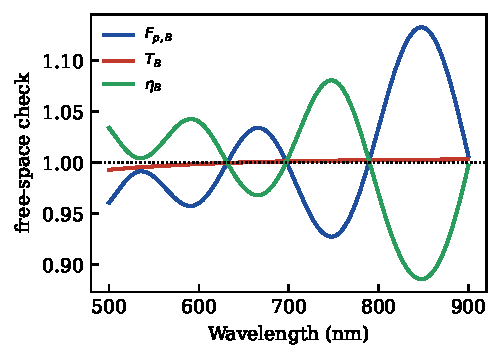
\includegraphics[width=0.48\linewidth]{fig_freespace.pdf}
\caption{Free-space reference B of the three-dimensional solver.}\label{fig:fs}\end{figure}
\begin{figure}[h]\centering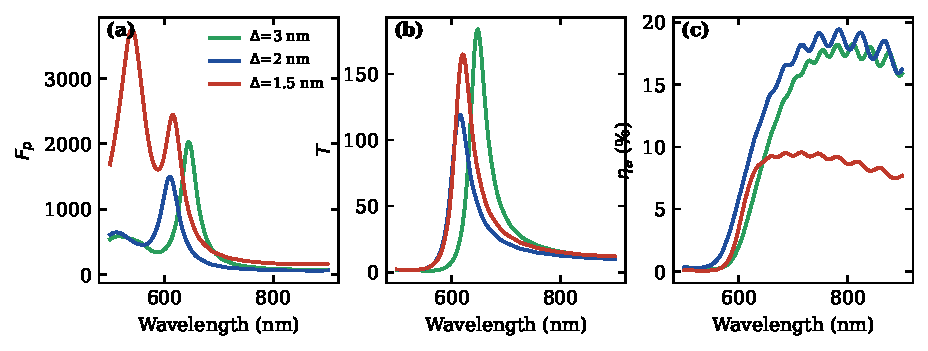
\includegraphics[width=\linewidth]{fig_mesh_lumerical.pdf}
\caption{Mesh sensitivity of case A in the three-dimensional solver: (a) $F_p$, (b) $T$, (c) $\eta_a$ for override
meshes of 3, 2 and 1.5~nm.}\label{fig:mesh}\end{figure}

\section*{S4. Body-of-revolution solver: method and benchmarks}
Cylindrical-coordinate FDTD (Meep~[2]) with field dependence $e^{im\varphi}$; axial dipole: $E_z$ source, $m=0$;
transverse dipole: $E_r$ source, $m=1$. $T$ is the ratio of the fluxes through a closed surface (top and bottom discs and a cylindrical side wall) around
the particle with and without it. $F_p=(P_{\rm rad}+P_{\rm abs})/P_0$, where $P_{\rm abs}$ is the net inflow through a
second closed surface that encloses only the particle, its top disc lying at mid-gap. The local density of states
at the source cell gives the same order of magnitude but is spiky near the metal and is used only as a cross-check. The band
\SIrange{490}{900}{nm} is assembled from three runs with pulses covering \SIrange{460}{610}{}, \SIrange{540}{760}{}
and \SIrange{630}{990}{nm}, of which only \SIrange{490}{570}{}, \SIrange{570}{700}{} and \SIrange{700}{900}{nm} are
kept: a broadband single run produced errors up to \SI{37}{\percent} at the band edges, where the source spectrum
is weak. Run time 30~\si{\micro\metre}/$c$ after the source (identical $F_p$ to 60); PML thickness
\SI{0.15}{\micro\metre}, with a \SI{0.3}{\micro\metre} check at the finest grid. To avoid long-lived numerical ringing,
the Lorentz-pole damping in the gold fit is bounded below by \SI{0.2}{\micro\metre^{-1}} (same fit accuracy).

Benchmark against the exact Mie solution for a dielectric sphere ($\varepsilon=4$, $R=\SI{15.874}{nm}$, radial dipole
at \SI{5}{nm}): a grid of \SI{2}{nm} reproduces $F_p$ within \SI{1}{\percent} in the band centres; a \SI{4}{nm} grid
gives a uniform \SIrange{4}{5}{\percent} overestimate with a maximum deviation of \SI{12}{\percent}. For gold (radial dipole, \SI{5}{nm} gap) at a \SI{2}{nm} grid, $T$ deviates from Mie by about
\SI{10}{\percent} while the power-balance $F_p$ is about three times too large; at a \SI{20}{nm} gap the $F_p$
error drops to \SI{24}{\percent} and $T$ agrees within \SI{5}{\percent}. The $F_p$ error is therefore a near-field
discretisation error of the staircased metal surface. Grids of 2, 1.33 and \SI{1}{nm} with linear extrapolation to
zero spacing are summarised in Table~\ref{tab:bor}.

\begin{table}[h]\centering
\caption{Body-of-revolution solver against exact Mie theory (gold sphere, radial dipole, \SI{5}{nm} gap) and grid
convergence of the nanorod (axial dipole, \SI{5}{nm} gap). Errors are medians over \SIrange{490}{900}{nm}.}\label{tab:bor}
\begin{tabular}{lcccc}\toprule
grid (nm) & sphere: $|\Delta F_p|$ & sphere: $|\Delta T|$ & rod: $T_{\max}$ ($\lambda_T$) & rod: NA 0.9 fraction\\\midrule
2.00 & 215\% & 10.2\% & 149 (631 nm) & 0.181\\
1.33 & 108\% & 8.4\% & 134 (617 nm) & 0.181\\
1.00 & 93\% & 7.2\% & 125 (611 nm) & 0.180\\
extrapolated & 48\% & 4.4\% & -- & --\\\bottomrule
\end{tabular}\end{table}

PML thickness 0.15 versus \SI{0.3}{\micro\metre} at the \SI{1}{nm} grid changes $T$ by \SI{0.1}{\percent} (median)
but $F_p$ by \SI{9}{\percent}. The radiative quantities are therefore converged to the level quoted in the main text,
whereas $F_p$ in a \SI{5}{nm} gap is not converged at grids of \SI{1}{nm} with a staircased surface and is not used.
The transverse ($m=\pm1$) configuration with a single $E_r$ source on the axis gave unphysical (negative) total
rates and is likewise not used; transverse results are taken from the three-dimensional solver. All runs were
executed on GitHub-hosted runners (workflow \texttt{.github/workflows/meep-runs.yml}); raw outputs are in
\texttt{isi/results/ci}.

\section*{References}
\noindent[1] P. B. Johnson and R. W. Christy, Phys. Rev. B \textbf{6}, 4370 (1972).\\
\noindent[2] A. F. Oskooi \emph{et al.}, Comput. Phys. Commun. \textbf{181}, 687 (2010).
\end{document}
